\documentclass{article}

\usepackage{fancyhdr}
\usepackage{extramarks}
\usepackage{amsmath}
\usepackage{amsthm}
\usepackage{amsfonts}
\usepackage{tikz}
\usepackage[plain]{algorithm}
\usepackage{algpseudocode}
\usepackage{enumerate}

\usepackage{listings}
\usepackage{xcolor}
\usepackage{forest}
\usepackage[shortlabels]{enumitem}
\setlist[enumerate, 1]{1\textsuperscript{o}}
\lstset { %
    language=bash,
        backgroundcolor=\color{black!5}, % set backgroundcolor
            basicstyle=\footnotesize,% basic font setting
}

%\usetikzlibrary{automata,positioning}
\usetikzlibrary{positioning,shapes,shadows,arrows,automata}

%
% Basic Document Settings
%

\topmargin=-0.45in
\evensidemargin=0in
\oddsidemargin=0in
\textwidth=6.5in
\textheight=9.0in
\headsep=0.25in

\linespread{1.1}

\pagestyle{fancy}
\lhead{\hmwkAuthorName}
\rhead{ (\hmwkClassInstructor\ \hmwkClassTime): \hmwkTitle}
\lfoot{\lastxmark}
\cfoot{\thepage}

\renewcommand\headrulewidth{0.4pt}
\renewcommand\footrulewidth{0.4pt}

\setlength\parindent{0pt}

\setcounter{secnumdepth}{0}
\newcounter{partCounter}


\newcommand{\hmwkTitle}{Portfolio submission, Topic 10}
\newcommand{\hmwkDueDate}{June 3, 2016}
\newcommand{\hmwkClass}{CS510 Languages and Low Level Programming}
\newcommand{\hmwkClassTime}{Spring 2016}
\newcommand{\hmwkClassInstructor}{Mark P. Jones}
\newcommand{\hmwkAuthorName}{Konstantin Macarenco}


\title{
    \vspace{2in}
    \textmd{\textbf{\hmwkClass:\ \hmwkTitle}}\\
        \normalsize\vspace{0.1in}\small{Due\ on\ \hmwkDueDate\ at 11:59pm}\\
        \vspace{0.1in}\large{\textit{\hmwkClassInstructor\ \hmwkClassTime}}
    \vspace{3in}
}

\author{\textbf{\hmwkAuthorName}}
\date{}

\renewcommand{\part}[1]{\textbf{\large Part \Alph{partCounter}}\stepcounter{partCounter}\\}

\begin{document}

\maketitle

\pagebreak

%\begin{enumerate}[(a), leftmargin = 0.7cm, nosep]
        \section{Topic 10.  Use practical case studies to evaluate and compare language design proposals.}

%STARTSTART

        With the lack of specific language for Low Level Programming, I picked two languages with
        Parallel Programming in mind (General C + MPI library, and Chapel - new domain specific
        language for parallel programming created by Cray).  Even though domain is different it
        shows that language designed for a specific domain can drastically aid applications
        development.
        Parallel programming complexity is similar, if not greater than
        LLP, with many potential issues on the top of regular mistakes like concurrency issues
        such as race conditions, deadlocks etc.
        MPI - message passing interface is a well known standard for external parallel computing.
        Chapel  is a modern high level language that hides
        all the intricacies of Message Passing. Chapel syntax is similar to Python, it is
        very expressive, safe, and has abstraction for many parallel programming approaches.
        Though Chapel is very different than C it uses C/MPI as an intermediate layer, i.e.
        first it compiles to C, hence the choice of comparison.\\
    
        I Compare implementation of Jacobi-Laplace algorithm in C/MPI vs Chapel. 
        
        \subsection{Problem Description}
        Jacobi-Laplace is a
        simple approach for solving Laplace equation with, used in many
        scientific applications, it is slow but highly parallelizable. 
        Laplace equation : 
        ${\phi^{t+1}}_{i,j} = \cfrac{1}{4} ({\phi^{t}}_{i+1,j} + {\phi^{t}}_{i-1,j} +
        {\phi^{t}}_{i,j+1} + {\phi^{t}}_{i,j-1}), 0 < i, j< N$ , i.e. current cell in a matrix is
        equal to a quarter of the sum of it's neighboring cells.\\
    
        The main problem with external is matrix partitioning, and message passing when computing
        border elements (image on the right).\\

                \begin{figure}[h]
                \caption{Element calculation on the left, MPI problem on the right (when
                matrix partitioned communication required among border layers)}
                    \vspace{0.3cm}
                    \centering
                    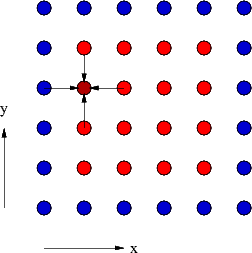
\includegraphics[width=0.40\textwidth]{jacobi.png}
                    \hspace{1.5cm}
                    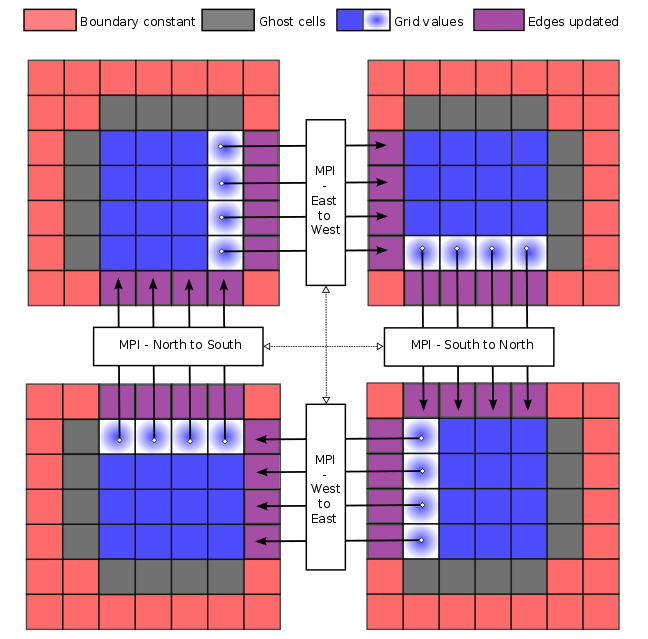
\includegraphics[trim=17 0 0 10mm, width=0.40\textwidth]{heat2d_mpi.png}
                \end{figure}
        

        \pagebreak

        \subsection{Language Comparison, based upon Jacobi-Laplace implementation (included)}
        \begin{centering}
        \begin{table}[h!]
            \centering
            \caption{Languages comparison}
            \label{my-label}
            \begin{tabular}{l| p{7.5cm} | p{7.5cm}} \hline
              Types             &  C/MPI & Chapel \\ \hline
              Complexity 
                    & High. It is quite a challenging task to do implement distributed Laplace in C/MPI, since matrix
                    mapping to the network done manually, and all border communications are
                    defined manually as well.
                    The particular implementation I use as an example, divides matrix to 4 regions,
                    each region is then sent to a remote CPU. It would be even more challenging to 
                    implement dynamic scalable matrix partitioning.  

                    &  Low. As easy as implementing sequential version, just need to
                        specify domain mapping. Chapel sequential and MPI implementations are almost
                        identical, with one exception - matrix needs to be mapped to the distributed
                        cluster. This is a natively supported operation in Chapel, short and
                        concise. Unlike C doesn't require any math, or matrix offsets calculation.
                        Code is simple and easy to read. Chapel includes multiple flexible
                        partitioning schemes, and also allows custom defined schemes. The problem is
                        mapped to the cluster automatically depending on the number of the available remote CPUs.
                    
                    \\ \hline
              Typing 
                  & Weak. C allows unsafe type cast, any type can be converted to any
                  other type  C MPI interface, is limited to sending empty types (*void) so
                  casting is required.
                  & Strong. It is strong the sense that typing error are prevented at runtime with
                  little implicit type conversion, and also utilizes static type checking.
                  All border communication's are implicitly type checked during runtime. 
                  \\ \hline
              Effort     
                  &  High.  
                    Large $\approx 620\ lines$ with comments
                    &  Low.
                    Small $\approx 60\ lines$ with comments
                \\ \hline
              Performance   
                & High. Area where C shines is performance. C implementation is up to x40 times
                faster.
                & Low. At this point of time Chapel suffers from performance issues. It is a new
                language, that is still undergoing major development, so intermediate C code produce by chapel
                compiler is far from being optimal. For example generated C code for the
                Laplace problem is $\approx 3K$ lines long \\ 
                \hline
              Abstraction 
                    & Low. Is one of the first ``high level languages'' is still very
                    close to bare metal (No OOP, First order functions, Garbage Collection etc.) 
                    & High. Support most of the modern abstractions, and new abstractions for
                    parallel programming, which makes conversion of sequential version of the
                    algorithm trivial.
                    \\ \hline
              Expressiveness 
                  & Low. C is well known for being hard to understand - unclear
                  syntax - subtle change in word ordering can cause unexpected behaviour, the
                  same symbol used for multiple purposes.
                  &  High. 
                  \\ \hline
              DS Features 
                  & Low. C is general purpose language, however it has been around
                  long enough to have wide support and reach set of third party libraries,
                  like MPI.
                  & High. Chapel was specifically created for aiding Parallel Programming
                  development easy, it supports most of the approaches out of the box (Shared
                  Memory, Message Passing, Data parallelism).
                  \\ \hline
              Modularity 
                  & Medium. 
                  & High. 
                  \\ \hline
              Simplicity 
                  & Medium. 
                  & High. 
                  \\ \hline
              Optimization 
                  & High. C 
                  & High. 
                  \\ \hline


            \end{tabular}
        \end{table}
        \end{centering}

        \textbf{Both implementations are included to the submission}. Files included: 

        \begin{itemize}
            \item laplace-mpi.c - C/MPI
            \item chapel-distr.chpl - Chapel
            \item Makefile
            \item laplace-distr.c - Chapel Generated code (not to be compiled or executed).
            \item chpl-prep - Environment setup for running chapel applications.
            \item mpi-prep - Environment setup required for running MPI applications.
            \item mpihosts - Set of available hosts in the Linuxlab cluster.
        \end{itemize}
        \subsection{Building and running}
        
        The code intended to be build on linuxlab machines.
        \begin{lstlisting}
make all
# MPI -
    source mpi-prep && mpirun -n 4 laplace-mpi  # number of remote procs must be 4 for 
        this application
# Chapel
    source chpl-prep && ./laplace-distr -nl [number of remote procs] # number of 
        procs can not exceed 20 
        \end{lstlisting}



%ENDEND
\end{document}
